\documentclass[conference]{IEEEtran}
\IEEEoverridecommandlockouts

\usepackage{cite}
\usepackage{amsmath,amssymb,amsfonts}
\usepackage{graphicx}
\usepackage{booktabs}
\usepackage{url}

\newcommand{\eps}{\epsilon}

\begin{document}

\title{A Behavioral Comparison of Adversarially Trained ResNet-18 and ViT-Tiny on CIFAR-10:\\ Transfer Metrics, Gradient Structure, and Layer-wise Feature Drift}

\author{\IEEEauthorblockN{\c{C}a\u{g}r{\i} \c{S}ahin}
\IEEEauthorblockA{\textit{Department of Software Engineering}\\
\textit{F{\i}rat University}\\
Elaz{\i}\u{g}, Turkey\\
csahin@firat.edu.tr}
\and
\IEEEauthorblockN{\"Ozal Y{\i}ld{\i}r{\i}m}
\IEEEauthorblockA{\textit{Department of Software Engineering}\\
\textit{F{\i}rat University}\\
Elaz{\i}\u{g}, Turkey}
}

\maketitle

\begin{abstract}
How convolutional neural networks (CNNs) and Vision Transformers (ViTs) differ under adversarial attack is usually summarized by a single robust-accuracy number. This paper reports preliminary results from an ongoing behavioral comparison of adversarially trained ResNet-18 and ViT-Tiny on CIFAR-10, evaluated with AutoAttack on the full test set at $\eps=8/255$, arguing that the single number hides most of the story. First, although the CNN attains higher absolute robust accuracy (35.74\% vs 32.94\%, McNemar $p<10^{-11}$), a conditional decomposition shows the picture is view-dependent: the PGD-10 gap traces entirely to the clean-accuracy gap, the per-model conditional ordering under AutoAttack slightly favors the ViT, yet on the jointly solved sample subset the CNN retains a significant edge. Second, the apparent cross-architecture transfer asymmetry depends strongly on the conditioning protocol: the raw metric manufactures an 8.3-point asymmetry, target-conditioned rates are statistically equivalent, while both-correct and successful-source protocols reveal a significant 5.3-point CNN-to-ViT advantage---protocol choice can create, erase, or reverse directional conclusions. Third, scale-invariant measures show modestly sparser CNN input gradients and higher ViT cross-sample gradient alignment in absolute---but not signed---cosine. Fourth, under attack, ViT features drift with an early-drop, mid-network-plateau profile, unlike the CNN's monotonic depth profile. Results are from a single training run per architecture and should be read as preliminary; an extended analysis is in preparation.
\end{abstract}

\begin{IEEEkeywords}
adversarial robustness, adversarial training, CIFAR-10, convolutional neural networks, transfer attacks, Vision Transformer
\end{IEEEkeywords}

\section{Introduction}
Deep image classifiers are vulnerable to adversarial examples---small, carefully crafted perturbations that flip predictions with high confidence~\cite{szegedy2014intriguing, goodfellow2015explaining}. As Vision Transformers (ViTs)~\cite{dosovitskiy2021image} join convolutional neural networks (CNNs)~\cite{he2016deep} as a dominant architecture family, a natural question is how the two families differ under attack. Much of the literature approaches this as a contest, reporting which architecture attains higher robust accuracy~\cite{bai2021transformers, benz2021adversarial, ali2024adversarial}. This paper takes a different, behavioral view: for a fixed pair of adversarially trained models, \emph{how} do the architectures differ---in what the headline robustness number is composed of, in how adversarial examples transfer between them, in the structure of their input gradients, and in how perturbations propagate through their layers?

We report preliminary results from an ongoing study of this question on CIFAR-10~\cite{krizhevsky2009learning}, using a ResNet-18 and a ViT-Tiny trained with the same adversarial objective and threat model and evaluated with AutoAttack~\cite{croce2020reliable} on the full test set. Our contributions are: (i) a conditional decomposition of robust accuracy showing that the ``CNN is more robust'' headline is composition-dependent; (ii) a multi-protocol transfer analysis showing that the measured direction and size of cross-architecture transfer asymmetry depend on the conditioning protocol---a methodological caution for transfer studies; (iii) paired, scale-invariant gradient-structure comparisons including a signed/absolute alignment distinction; and (iv) a layer-wise feature-drift comparison revealing qualitatively different depth profiles. All results derive from per-sample-logged evaluations; results are from a single training run per architecture and should be read as preliminary.

\section{Related Work}
Adversarial examples and gradient-based attacks were established by Szegedy et al.~\cite{szegedy2014intriguing} and Goodfellow et al.~\cite{goodfellow2015explaining}; projected gradient descent (PGD) adversarial training~\cite{madry2018towards} remains the standard defense, with robust overfitting and early stopping characterized by Rice et al.~\cite{rice2020overfitting}. AutoAttack~\cite{croce2020reliable} and RobustBench~\cite{croce2021robustbench} standardized robustness evaluation.

Direct CNN--ViT robustness comparisons include Bai et al.~\cite{bai2021transformers}, who found that under fair recipes transformers are not more adversarially robust than CNNs, and Benz et al.~\cite{benz2021adversarial}. Closest to our setting, Ali et al.~\cite{ali2024adversarial} compared the robustness of standardly trained ViTs and CNNs under FGSM, PGD, and DeepFool score comparisons. Our study differs in three ways: both models are \emph{adversarially trained} under a matched objective, evaluation uses full-test AutoAttack with paired per-sample statistics, and the comparison goes beyond scores to conditional decompositions, protocol-explicit transfer, gradient structure, and layer-wise drift. ViT adversarial training is known to be recipe-sensitive on small datasets~\cite{mo2022adversarial, debenedetti2023light}, and with specialized augmentation ViTs can surpass WideResNets on CIFAR-10~\cite{wu2025vision}; our conclusions therefore hold under the baseline recipe we study, not for optimally trained ViTs.

For transfer evaluation, conditioning on correctly classified samples is established practice~\cite{liu2017delving, dong2018boosting, mahmood2021robustness, ravikumar2023trend}, with both-correct variants used by Mahmood et al.~\cite{mahmood2021robustness} and TREND~\cite{ravikumar2023trend}. Our contribution is to show on a single dataset that the \emph{choice} among these protocols qualitatively changes the asymmetry conclusion.

\section{Method}
\subsection{Models and Training}
We compare ResNet-18 (11.2M parameters; CIFAR-style stem) and ViT-Tiny (5.7M parameters; \texttt{timm}~\cite{rw2019timm} architecture with $16\times16$ patches on inputs bilinearly upsampled to $224\times224$), both trained from scratch on CIFAR-10 with basic augmentation and then adversarially fine-tuned. Adversarial training minimizes a mixed objective $(1-\lambda)\mathcal{L}_{CE}(f(x),y) + \lambda\,\mathcal{L}_{CE}(f(x_{adv}),y)$ with $\lambda=0.5$, where $x_{adv}$ is generated by PGD-10 ($\eps=8/255$, $\alpha=2/255$) in training mode, following standard practice~\cite{madry2018towards, rice2020overfitting}. Fine-tuning uses low learning rates ($10^{-3}$; SGD for the CNN, AdamW~\cite{loshchilov2017decoupled} for the ViT) and early stopping on a held-out 2{,}000-sample validation split; the test set is used only for final evaluations. As an upper reference we include the WideResNet-28-10 checkpoint of Gowal et al.~\cite{gowal2020uncovering} from RobustBench~\cite{croce2021robustbench}; it is trained with additional data and a stronger recipe, so we keep it visually and analytically separate from the matched pair.

\subsection{Evaluation and Metrics}
All evaluations use the full 10{,}000-sample test set with per-sample outcomes logged. Robustness is measured with FGSM, PGD-10, and the standard AutoAttack ensemble at $\eps=8/255$. Beyond absolute robust accuracy, we report the \emph{conditioned fooling rate} (fraction of clean-correct samples flipped by the attack); since clean-misclassified samples count as non-robust, absolute robustness factorizes exactly as $\text{robust} = \text{clean} \times (1-\text{cond.\ fooling})$, separating a clean-accuracy component from a conditional-susceptibility component. We additionally evaluate the \emph{both-correct} subset (samples both models classify correctly), which yields exactly paired comparisons.

For transfer, adversarial examples crafted on a source model are evaluated on the other (target) model under three conditioning protocols: \emph{target-correct} (target classifies the clean sample correctly), \emph{both-correct}~\cite{mahmood2021robustness, ravikumar2023trend}, and \emph{successful-source} (target-correct and the attack succeeded on the source). Confidence intervals are percentile bootstrap (10{,}000 resamples); paired protocol comparisons use sign-flip permutation tests and two one-sided equivalence tests (TOST).

Gradient structure is analyzed on 500 fixed test samples with per-sample loss gradients: scale-invariant sparsity (Hoyer, Gini~\cite{hurley2009comparing}, and the fraction of components below 1\% of the per-sample maximum) with per-sample paired Wilcoxon tests (Holm-corrected), and cross-sample gradient alignment as the mean absolute cosine over all sample pairs, with the signed mean reported alongside. Layer-wise feature drift compares clean and adversarial representations per block (cosine similarity, norm change) for the ViT's 12 transformer blocks and the CNN's 8 residual blocks ($n$=100).

\section{Results}
\subsection{Robustness: One Headline, Three Readings}
Table~\ref{tab:main} and Fig.~\ref{fig:rob} give absolute results: the adversarially trained CNN leads the ViT under every attack (AutoAttack 35.74\% vs 32.94\%; McNemar on shared samples $\chi^2=48.65$, $p<10^{-11}$), and both trail the reference WideResNet, whose advantage reflects capacity, extra data, and a stronger recipe jointly~\cite{gowal2020uncovering}. Fig.~\ref{fig:eps} shows the gap is stable across perturbation budgets.

\begin{table}[!t]
\centering
\caption{Robustness on the full CIFAR-10 test set ($\eps=8/255$).}
\label{tab:main}
\footnotesize
\setlength{\tabcolsep}{4pt}
\begin{tabular}{lccccc}
\toprule
\textbf{Model} & \textbf{AT} & \textbf{Clean} & \textbf{FGSM} & \textbf{PGD-10} & \textbf{AA} \\
\midrule
ResNet-18 & -- & 94.37 & 30.93 & 0.01 & -- \\
ViT-Tiny & -- & 77.50 & 3.34 & 0.03 & -- \\
ResNet-18 & \checkmark & 85.42 & 49.90 & 40.97 & \textbf{35.74} \\
ViT-Tiny & \checkmark & 75.65 & 40.07 & 36.09 & \textbf{32.94} \\
\midrule
WRN-28-10$^{\dagger}$ & \checkmark & 89.48 & 70.91 & 66.92 & 62.76 \\
\bottomrule
\multicolumn{6}{l}{\scriptsize $^{\dagger}$External reference checkpoint~\cite{gowal2020uncovering}: stronger recipe and}\\
\multicolumn{6}{l}{\scriptsize \phantom{$^{\dagger}$}additional data; AA value as reported by RobustBench.}
\end{tabular}
\end{table}

\begin{figure}[!t]
\centering
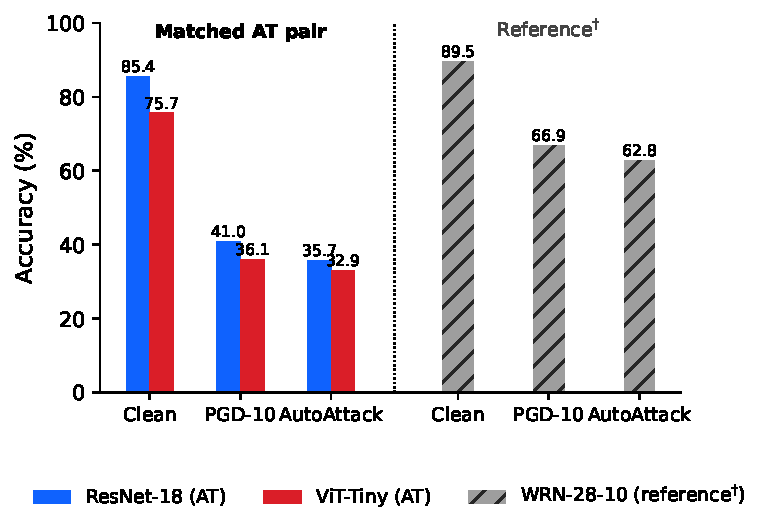
\includegraphics[width=\columnwidth]{figures/fig_b1_robustness.pdf}
\caption{Clean, PGD-10, and AutoAttack accuracy. The matched adversarially trained pair (left) is the object of study; WRN-28-10 (right, hatched) is an external reference trained with a stronger recipe and extra data.}
\label{fig:rob}
\end{figure}

\begin{figure}[!t]
\centering
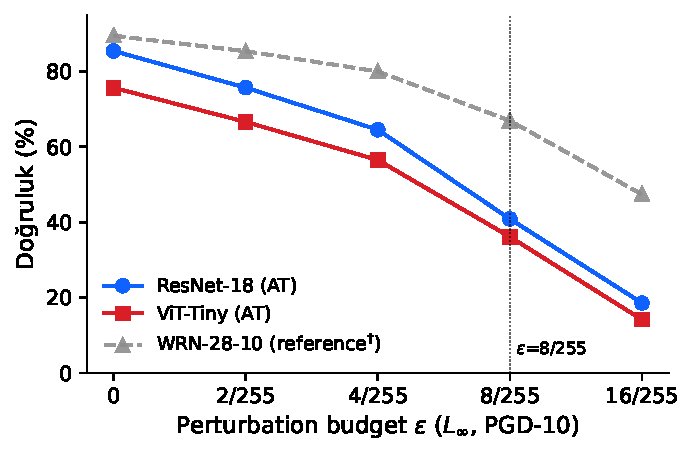
\includegraphics[width=\columnwidth]{figures/fig_b2_eps_sweep.pdf}
\caption{PGD-10 accuracy vs.\ perturbation budget (full test set). The reference model is drawn dashed and gray to keep it visually distinct from the matched pair.}
\label{fig:eps}
\end{figure}

The conditional decomposition (Table~\ref{tab:cond}) changes the reading. Under PGD-10 the two models' conditioned fooling rates are statistically indistinguishable (52.15\% vs 52.33\%), so the absolute PGD gap is fully accounted for by clean accuracy ($85.42 \times 0.478$ vs $75.65 \times 0.477$). Under AutoAttack the per-model conditional ordering even reverses slightly in the ViT's favor (58.16\% vs 56.46\% fooling). Yet on the 7{,}260 jointly solved samples---an exactly paired comparison---the CNN stays significantly ahead under both attacks (PGD 54.92\% vs 49.61\%, McNemar $p<10^{-20}$; AA 48.15\% vs 45.33\%, $p<10^{-6}$). These views reconcile compositionally: the $\sim$1{,}300 samples only the CNN solves cleanly are almost never robust (below 8\% PGD survival), diluting its per-model conditional rate. A single robust-accuracy number would hide all of this structure.

\begin{table}[!t]
\centering
\caption{Conditional decomposition (full test set; 95\% bootstrap CIs). Both-correct: the $n$=7{,}260 samples both models classify correctly.}
\label{tab:cond}
\scriptsize
\setlength{\tabcolsep}{2.5pt}
\begin{tabular}{lcccc}
\toprule
& \multicolumn{2}{c}{\textbf{Cond.\ fooling (\%)}} & \multicolumn{2}{c}{\textbf{Both-correct robust (\%)}} \\
\textbf{Model} & \textbf{PGD-10} & \textbf{AA} & \textbf{PGD-10} & \textbf{AA} \\
\midrule
ResNet-18 AT & 52.15 [51.1, 53.2] & 58.16 [57.1, 59.2] & \textbf{54.92} & \textbf{48.15} \\
ViT-Tiny AT & 52.33 [51.2, 53.5] & \textbf{56.46} [55.4, 57.6] & 49.61 & 45.33 \\
\bottomrule
\end{tabular}
\end{table}

\subsection{Transfer: the Protocol Is Part of the Result}
Table~\ref{tab:protocols} reports cross-architecture transfer under three established conditioning protocols. The raw (unconditioned) rates would suggest an 8.3-point asymmetry favoring CNN sources (40.2\% vs 31.9\%)---an artifact of the targets' ten-point clean-accuracy difference. The target-correct protocol removes this confound and shows near-parity (difference 0.63 points; TOST-equivalent within $\pm$2 points, $p=0.016$), and this parity is stable under the momentum-based MI-FGSM~\cite{dong2018boosting} (19.85\% vs 20.11\%). However, the both-correct and successful-source protocols \emph{reverse the conclusion again}, revealing a significant $\sim$5.3-point CNN$\rightarrow$ViT advantage on jointly solved samples (paired bootstrap CI [4.39, 6.25]; sign-flip permutation $p<5\times10^{-5}$; TOST equivalence rejected even at $\pm$3 points). The mechanism is compositional: samples the target solves cleanly but the source does not are hyper-vulnerable in both directions (56.9\% and 63.0\% fooling), and their asymmetric counts (1{,}282 vs 305) pull the target-correct rates to parity. The practical lesson for cross-architecture transfer studies: the conditioning protocol can create, erase, or reveal a directional difference on the same data, so it must be stated explicitly and, where feasible, varied.

\begin{table}[!t]
\centering
\caption{Transfer asymmetry under three conditioning protocols (PGD-10, $\eps$=8/255, full test set; 95\% bootstrap CIs).}
\label{tab:protocols}
\scriptsize
\setlength{\tabcolsep}{3pt}
\begin{tabular}{lccc}
\toprule
\textbf{Protocol} & \textbf{CNN$\rightarrow$ViT} & \textbf{ViT$\rightarrow$CNN} & \textbf{Diff.} \\
\midrule
Target-correct & 20.95 [20.03, 21.88] & 20.32 [19.47, 21.19] & $+$0.63 \\
Both-correct & 19.19 [18.26, 20.10] & 13.86 [13.07, 14.66] & $+$5.33 \\
Successful-source & 39.07 [37.47, 40.66] & 33.79 [32.48, 35.13] & $+$5.28 \\
\bottomrule
\end{tabular}
\end{table}

\subsection{Gradient Structure}
On 500 fixed test samples measured under both models, CNN input gradients are consistently but modestly sparser than the ViT's on all three scale-invariant measures (Hoyer 0.474$\pm$0.009 vs 0.449$\pm$0.011; Gini 0.634 vs 0.606; 31.5\% vs 25.8\% of components below 1\% of the per-sample maximum), with paired Wilcoxon tests highly significant (Holm-corrected $p<10^{-15}$) at small-to-medium effect sizes (paired Cohen's $d$ 0.34--0.65). Interestingly, this ordering is created by adversarial training: the clean-trained ViT is the sparser model (Hoyer 0.406 vs 0.354), consistent with the strong sparsifying effect of adversarial training on CNN gradients~\cite{chalasani2020concise}. Cross-sample gradient alignment is higher for the ViT in mean absolute cosine over all pairs (0.052 vs 0.038; nearly identical in the clean-trained counterparts, indicating an architectural rather than training-induced property), but the \emph{signed} mean cosine is near zero for both ($\leq$0.002): samples share sensitivity axes, not consistent directions.

\subsection{Layer-wise Feature Drift}
Fig.~\ref{fig:drift} compares how far each block's representation of an attacked input drifts from its clean counterpart. The ViT shows an early-drop, mid-network-plateau profile: cosine similarity falls quickly to a minimum of 0.955 at Block~8, then mildly recovers (0.965 at Blocks~10--11), with feature norms changing by less than 1.5\% throughout---the perturbation corrupts representation \emph{direction}, not magnitude. The CNN behaves qualitatively differently: cosine similarity declines monotonically and acceleratingly with depth (0.995 down to 0.913 at the final residual block), with large terminal norm distortions ($-$6.4\% and $+$7.2\% in the last two blocks). The plateau-and-recovery shape is thus specific to the evaluated ViT rather than a generic deep-network property, extending layer-wise representation analyses of clean-trained ViTs~\cite{raghu2021vision} to the adversarially trained setting.

\begin{figure}[!t]
\centering
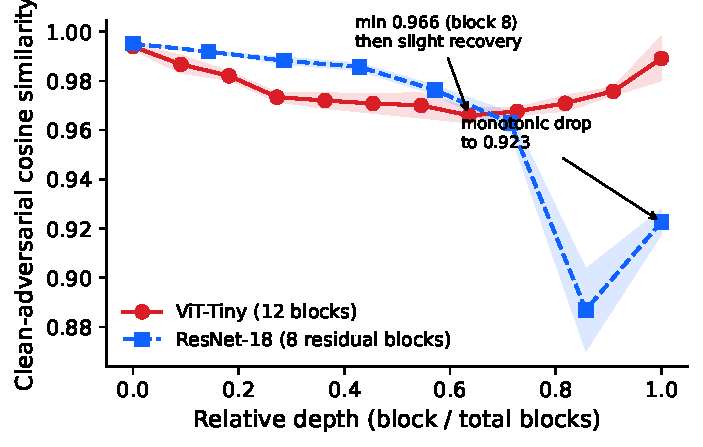
\includegraphics[width=\columnwidth]{figures/fig_b3_feature_drift.pdf}
\caption{Clean--adversarial cosine similarity by relative depth under white-box PGD-10 ($n$=100). ViT: early drop, mid-network minimum, mild recovery. CNN: monotonic, accelerating decline with large terminal norm distortion.}
\label{fig:drift}
\end{figure}

\section{Discussion and Limitations}
Three takeaways emerge. First, single-number robustness comparisons are lossy: our conditional decomposition supports simultaneously ``the CNN is more robust'' (absolute, both-correct), ``conditional susceptibility is matched'' (per-model PGD), and ``the ViT loses less on its solved samples'' (per-model AutoAttack). Second, transfer asymmetry claims are protocol-relative; cross-architecture studies should report their conditioning protocol as part of the result. Third, the architectures differ behaviorally in gradient concentration and in where along the depth adversarial damage accumulates, suggesting differently placed stabilization for each.

Several limitations bound these conclusions. Results are from a single training run per architecture under one baseline recipe and should be read as preliminary; ViT robustness is known to be recipe-sensitive~\cite{mo2022adversarial, debenedetti2023light, wu2025vision}. The study covers one dataset, one model pair, and the $L_\infty$ threat model at a single budget for the conditional analyses. The gradient and drift measurements are behavioral correlates, not established causal explanations. An extended analysis addressing training-seed variance, additional transfer attacks, and spatial gradient statistics is in preparation.

\section{Conclusion}
For a matched adversarially trained ResNet-18/ViT-Tiny pair on CIFAR-10, we showed that the robustness headline is composition-dependent, that measured transfer asymmetry is largely a property of the conditioning protocol, that gradient-structure differences are consistent but modest (with alignment differences unsigned in nature), and that adversarial damage accumulates at qualitatively different depths in the two architectures. We offer these preliminary results as a template for protocol-explicit, multi-view robustness comparisons between architecture families.

\bibliographystyle{IEEEtran}
\bibliography{bildiri}

\end{document}
